\documentclass[14pt]{article}
\usepackage{amssymb}
\usepackage[english,russian]{babel}
\usepackage{tikz}
\linespread{1.6}
\usepackage{xcolor}
\usepackage{hyperref}
\usepackage{geometry}
\usepackage{amsmath}
\usepackage{graphicx}
%\graphicspath{{pictures/}}
\DeclareGraphicsExtensions{.pdf,.png,.jpg}
\linespread{1.6}
\geometry{
	paper=a4paper,
	top=3.5cm,
	bottom=2.5cm,
	right=2cm,
	left=3.5cm
}
\begin{document}
	\begin{titlepage}
		\begin{center}
			\large	Министерство науки и высшего образования Российской Федерации\\ НАЦИОНАЛЬНЫЙ ИССЛЕДОВАТЕЛЬСКИЙ ЯДЕРНЫЙ УНИВЕРСИТЕТ «МИФИ»\\
			ИНСТИТУТ ЯДЕРНОЙ ФИЗИКИ И ТЕХНОЛОГИЙ\\КАФЕДРА ТЕОРЕТИЧЕСКОЙ И ЭКСПЕРИМЕНТАЛЬНОЙ ФИЗИКИ ЯДЕРНЫХ РЕАКТОРОВ
			\vspace{0.25cm}
			
			
			\begin{flushright}
			\small{На правах рукописи}\\
           \small{ УДК 621.039.546.8}
			\end{flushright}
			\vfill
			
			\Huge Шодмонов Аббос
			\vfill
			{\Large РАЗРАБОТКА МЕТОДОВ АКТИВНОГО КОНТРОЛЯ ОБОГАЩЕНИЯ ТВС РЕАКТОРА ВВЭР – 1000\\
			}
			\bigskip
		\end{center}
	
		\begin{center} Выпускная квалификационная работа магистра\\
        Направление подготовки\\
         14.04.02 Ядерные физика и технологии
         \end{center}
         
         \vfill
         
         \begin{flushright}
                 Выпускная квалификационная\\
работа защищена\\
«» июня 2021 г.\\
Оценка \_\_\_\_\_\_\_\_\_\_\_\_\_ \\
Секретарь ГЭК \_\_\_\_\_\_\_\_\_\_\_\_ 
         \end{flushright}
		\vfill
		
		
		\begin{center}
			г. Москва\\ 2020
		\end{center}
	\end{titlepage}
	\newpage
	\renewcommand{\contentsname}{Содержание}
	\tableofcontents
	\newpage
	\section{Введение}
	\hspace{0.4cm}
	При обосновании безопасности межобъектового транспортирования
ОЯТ для каждой конкретной загрузки ТУК эксплуатирующей организации
необходимо доказать соблюдение установленных в нормативных документах
требований безопасности, ограничивающих установленными пределами
максимальные значения нормируемых показателей безопасности: уровней
мощности дозы на поверхности (за защитой) и на определенных расстояниях
от поверхностей упаковки и транспортного средства, тепловой нагрузки на
ТУК, допустимой потери радиоактивного содержимого из упаковки,
эффективного коэффициента размножения нейтронов и т.д. Это требует от
специалистов эксплуатирующей организации проведения целого ряда
сложных и трудоемких расчетов, реализующих всю цепочку перехода от
известных и/или измеряемых параметров (конструкции ТВС, длины и массы
топливного столба, начального обогащения, глубины выгорания, времени
выдержки и т. д.) к вышеперечисленным нормируемым показателям
безопасности: от расчета пространственного распределения по высоте ОТВС
радионуклидного
состава
ОЯТ,
его
характеристик,
как
источника
нейтронного и гамма – излучения, до расчета ослабления излучения в защите
ТУК и поиска точек на его поверхности и за ее пределами (априори
неизвестных), в которых достигается нормируемое максимальное значение
суммарной мощности дозы излучения.
Проведение таких расчетов является задачей, хоть и вполне реализуемой
при наличии у специалистов достаточных фундаментальных знаний,
расчетного
инструментария,
практического
опыта
выполнения
вышеупомянутых расчетов, но далеко не тривиальной. Накопленный опыт
показывает, что не всегда обоснование безопасности транспортирования
ОЯТ с энергоблоков АЭС на заводы регенерации выполняется безошибочно,
поскольку даже многократно выверенный алгоритм проведения расчетов не
позволяет избежать ошибок, связанных с человеческим фактором [1].
	
	Частично вышеописанную проблему позволяет решить действующий в
настоящее время отраслевой стандарт ОСТ 95 745–2005 [2]. В нем для ОТВС
реакторов ВВЭР–1000 и ВВЭР–440 различной номенклатуры консервативно
установлены
диапазоны
изменения
вышеупомянутых
измеряемых
параметров, при соответствии которым характеристик транспортируемых
ОТВС значения нормируемых показателей безопасности заведомо будут
удовлетворять
всем
требованиям
нормативных
документов.
Поэтому
проведение трудоемких и сложных расчетов конкретных значений этих
нормируемых
показателей
становится
ненужным
и
обоснование
безопасности транспортирования партии ОТВС сводится к простой проверке
выполнения соответствия измеряемых характеристик загружаемых в ТУК
ОТВС требованиям стандарта ОСТ 95 745–2005 [2].
Однако
консервативность
подхода,
реализованного
в
[2],
с
неизбежностью приводит к тому, что даже среди ТВС «традиционной»
номенклатуры всегда найдется несколько, параметры которых выходят за
переделы допустимых установленных отраслевым стандартом значений. Это
приводит к необходимости проведения полного расчетного обоснования
безопасности транспортирования ТУК, в составе которых требовалось
разместить хотя бы одну такую ОТВС (наряду с ОТВС, удовлетворяющих
требованиям ОСТ 95 745–2005 [2]). Частота таких ситуаций год от года
увеличивается
и
перед
специалистами
Федеральной
службы
по
экологическому, техническому и атомному надзору (далее – Ростехнадзор)
постоянно возникает задача оценивать достаточность представленных
эксплуатирующей
организацией
полных
расчетных
обоснований
безопасности.

Поэтому для повышения эксплуатационной надежности и безопасности
АЭС актуальным является расширение действующей в РФ системы подготовки
кадров за счет включения в нее комплекса программ и методик прямого
компьютерного моделирования и моделирования на аналитических тренажерах
аварийных
и
других
переходных
режимов,
освоение
которых
может
осуществляться как в компьютерных классах, оснащенных соответствующим
программным обеспечением под руководством инструктора, так и индивидуально
с использованием персонального компьютера.

\textbf{Объект исследования} – реактор ВВЭР-1000.

\textbf{Предмет исследования} – математические модели компьютерного и
методики
имитационного
моделирования
нейтронно-физических
и
теплогидравлических процессов энергоблока АЭС с реактором ВВЭР-1000.

\textbf{Цель работы} – повышение уровня безопасности управления ядерной
энергоустановкой посредством включения в действующую систему подготовки
кадров комплекса программ прямого компьютерного моделирования и методик
имитационного моделирования на аналитических тренажерах влияющих на
безопасность реактора переходных режимов.
	
	
	Одним из важнейших условий безопасной эксплуатации АЭС является формирование топливных  загрузок,  удовлетворяющих  требованиям  ядерной  безопасности.  Каждая  новая модель  тепловыделяющих  сборок  проходит  полный  цикл разработки,  испытаний  и исследований, включая обоснование безопасности топливных циклов на их основе.  
	
	Для  этого  проектными  организациями  при  разработке  новых  топливных  циклов определяется,   в   частности,   диапазон   изменения   основных   нейтронно-физических характеристик, влияющих на ядерную безопасность, так называемые «рамочные» параметры, которым в процессе эксплуатации должны соответствовать реальные топливные загрузки. 
	
	Формирование  и  нейтронно-физический  расчет  очередных  топливных  загрузок энергоблоков  с  реакторами  ВВЭР  производится  персоналом  АЭС  с  учетом  утвержденных графиков  ремонтов  и  выработки  электроэнергии.  Активные  зоны  комплектуются  типами ТВС,  содержащимися  в  технических  условиях  на  топливо  и  в  обоснованиях  безопасности. Номенклатура  ТВС  подпитки,  схемы  перегрузок  ТВС  выбираются  в  соответствии  с обоснованной в проекте общей стратегией топливного цикла. 
	
	Реальные  топливные  загрузки,  как  правило,  отличаются  от  проектных  топливных загрузок.  Эти  отличия  обусловлены  отклонениями  в  графике  выработки  электроэнергии  в связи с требованиями энергосистемы и различными эксплуатационными ограничениями. 
	
	Поэтому  возникает  необходимость  в  проверке  нейтронно-физических  характеристик текущих   топливных   загрузок   с   целью   подтверждения   их   соответствия   проектным требованиям   безопасности   («рамочным»   параметрам).   Выполнение   установленных ограничений  для  нейтронно-физических  характеристик является  одним  из  основных факторов для разрешения эксплуатации энергоблока на заявленной мощности. 
	
	Важность   контроля   нейтронно-физических   характеристик   текущих   топливных загрузок возрастает в период эксплуатации АЭС на повышенной мощности.  
	
	Контроль    выполнения    проектных    ограничений    для    нейтронно-физических характеристик текущих топливных загрузок российских реакторов ВВЭР возложен на ОАО «ВНИИАЭС».
	
	Основными  документами,  которые  используются  для  подтверждения  соответствия нейтронно-физических   характеристик   текущих   топливных   загрузок   установленным требованиям, являются руководящие документы эксплуатирующей организации; в частности для  ВВЭР-1000 −  «Номенклатура  эксплуатационных  нейтронно-физических  расчетов  и измерений для топливных загрузок ВВЭР-1000» (далее «Номенклатура...»). 
	
	Допустимые значения нейтронно-физических характеристик, содержащиеся в данных руководящих  документах,  определяются  исходя  из  требований  ТОБ  РУ,  ТОБ  АС  и  ТУ  на топливо и корректируются в соответствии с изменениями в проектной документации. 
	
	«Номенклатура...»  устанавливает  требования  к  формированию  топливных  загрузок, объему и результатам расчетов и измерений нейтронно-физических характеристик, включая вопросы  порядка  оформления  и  согласования  отчетных документов,  регламентирует необходимый  объем  измерений  и  порядок  сопоставления  их  результатов  с  расчетными  и проектными   данными.   Документ   распространяется   как   на   период   промышленной эксплуатации, так и на период опытной эксплуатации топлива, исключая первую топливную загрузку. 
	
	Расчеты,  выполняемые  в  соответствии  с  руководящим  документом,  содержат информацию   для   формирования   «Альбома   нейтронно-физических   характеристик», используемого  оперативным  персоналом  АЭС,  а  также  для  пополнения  банка  данных  по топливным  загрузкам  с  целью  обеспечения  возможности  оперативного  рассмотрения вопросов, связанных с безопасностью эксплуатации и использованием ядерного топлива. 
	
	Расчеты  нейтронно-физических  характеристик  на  российских  АЭС  проводятся квалифицированными  специалистами,  прошедшими  в  ОАО «ВНИИАЭС»  необходимую подготовку и аттестованными в соответствии с руководящим документом эксплуатирующей организации:   «Положение   о   порядке   проведения   аттестации   персонала   атомных электростанций   с   реакторами   ВВЭР,   выполняющего   нейтронно-физические   расчеты топливных загрузок». 
	
	\section{Общая характеристика реактора ВВЭР}
	\hspace{0.4cm}
	ВВЭР (Водо-Водяной Энергетический Реактор)— водо-водяной корпусной энергетический ядерный реактор с водой под давлением, представитель одной из наиболее удачных ветвей развития ядерных энергетических установок, получивших широкое распространение в мире. 
	
Общее название реакторов этого типа в других странах— PWR, они являются основой мировой мирной ядерной энергетики. Первая станция с таким реактором была запущена в США в 1957 году, АЭС Шиппингпорт. 

\begin{figure}
	    \centering
	    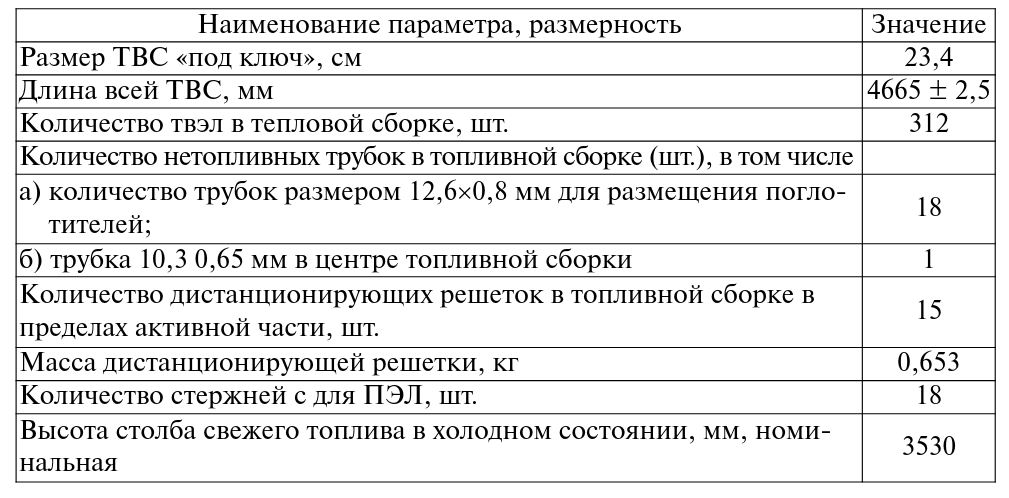
\includegraphics[width=\linewidth]{Picture6}
	    \caption{Основные характеристики корпуса ВВЭР}
	    \label{fig:my_label}
	\end{figure}

ВВЭР был разработан в СССР параллельно с реактором РБМК и обязан своим происхождением одной из рассматривающихся в то время реакторных установок для атомных подводных лодок. Идея реактора была предложена в Курчатовском институте С.М.Фейнбергом. Работы над проектом начались в 1954 году, в 1955 году ОКБ «Гидропресс» приступило к его разработке. Научное руководство осуществляли И.В.Курчатов и А.П.Александров[1]. 

Первый советский ВВЭР (ВВЭР-210) был введён в эксплуатацию в 1964 году на первом энергоблоке Нововоронежской АЭС. Первой зарубежной станцией с реактором ВВЭР-210 стала введённая в работу в 1966 году АЭС Райнсберг (ГДР). 

Создатели реакторов ВВЭР: 
\begin{itemize}
\item научный руководитель: Курчатовский институт (г.Москва)
\item разработчик: ОКБ «Гидропресс» (г. Подольск)[2].
\item изготовитель: Ижорские заводы (г. Санкт-Петербург), Атоммаш (г.Волгодонск, с начала 90-х до 2012 года производство реакторов было остановлено) и компания ŠKODA JS (Чехия, до начала 90-х)[3].
	\end{itemize}
	
	Направление ВВЭР разрабатывалось в СССР параллельно с РБМК. В начале 1950-х гг. уже рассматривались несколько вариантов реакторных установок для атомных подводных лодок. Среди них имелась и водо-водяная установка, идея которой была предложена в Курчатовском институте С.М.Фейнбергом. Этот вариант был принят и для разработки гражданских энергетических реакторов. Работы над проектом начались в 1954 году, в 1955 году ОКБ «Гидропресс» приступило к разработке конструкции. Научное руководство осуществляли И.В.Курчатов и А.П.Александров[5].
	
Первоначально рассматривались несколько вариантов, техническое задание на проектирование которых было представлено Курчатовским институтом к маю 1955 года. В их число входили: ВЭС-1— водо-водяной с алюминиевой активной зоной для низких параметров пара, ВЭС-2— с циркониевой активной зоной и повышенными параметрами пара, ЭГВ— водогазовый реактор с перегревом пара, ЭГ— газовый реактор с графитовым замедлителем. Также рассматривался вопрос о комбинировании в одном энергоблоке ВЭС-2 для производства насыщенного пара и ЭГ для перегрева этого пара. Из всех вариантов для дальнейшей разработки был выбран ВЭС-2[6][7]. 

В процессе научных изысканий конструкция ВЭС-2 была существенно изменена. Одной из основных причин этого стала поэтапная модификация ядерного топлива: первоначально предполагалась загрузка 110 тонн природного урана и 12-15 тонн с 25\% обогащением, но к 1957 году было принято решение использовать однородную активную зону с 1-3\% обогащением. Также полностью поменялась конструкция топливных сборок, изменились геометрические размеры реактора, увеличились многие теплотехнические параметры. Итоговый вариант установки с реактором ВВЭР-210 был реализован в 1964 году на Нововоронежской АЭС, ставшей первой АЭС с ВВЭР[8][9]. 
В 1970 году был запущен 2-й блок Нововоронежской АЭС с реактором ВВЭР-365, а в 1971 году— 3-й блок той же станции с реактором ВВЭР-440, который стал серийным советским реактором первого поколения. АЭС с ВВЭР-440 получили большое распространение, множество энергоблоков было построено как в СССР, так и в других странах. Первым проектом второго поколения, к которому относятся блоки с ВВЭР-1000, стал разработанный для атомной энергетики Финляндии проект энергоблока АЭС Ловииса с ВВЭР-440. В 1977 и 1980 году на этой станции было запущено два энергоблока, при создании которых использовались многие технические решения, в дальнейшем реализованные и в АЭС с ВВЭР-1000, например, железобетонная гермооболочка[5]. 

Работы по созданию ВВЭР-1000 начались в 1966 году, к 1969 году в Курчатовском институте было подготовлено техническое задание на проект установки, которое утвердил его научный руководитель А.П.Александров. К 1971 году проект ВВЭР-1000 был разработан ОКБ «Гидропресс» под руководством главного конструктора В. В. Стекольникова и утверждён Минсредмашем СССР[10][11]. 
Единичная мощность реакторов ВВЭР выросла с 440 до 1000 МВт за счёт увеличения площади теплообменной поверхности активной зоны, повышения энергонапряжённости топлива, увеличения расхода теплоносителя через реактор. Объём активной зоны был расширен примерно в 1,5 раза за счёт увеличения её высоты (условие возможностей транспортирования по железным дорогам СССР накладывало ограничения на поперечные размеры реактора). Однако мощность возросла более чем в 2 раза, что потребовало увеличения средней энергонапряжённости активной зоны примерно на 40 \%. При этом разработчикам удалось снизить коэффициенты неравномерности энерговыделения примерно на 30 \%. Скорость теплоносителя в реакторе возросла с 4,1 до 5,7 м/с, давление в первом контуре со 125 до 160 кгс/см$^{2}$[12][13]. 
Также были изменены некоторые технические решения, например, число петель циркуляции теплоносителя было уменьшено с шести в ВВЭР-440 до четырёх в ВВЭР-1000. Таким образом, мощность каждой петли стала 250 МВт вместо прежних 73 МВт. Соответственно, единичная мощность главных циркуляционных насосов (ГЦН), парогенераторов и другого основного оборудования возросла более чем в 3 раза. Диаметр основных трубопроводов первого контура вырос с 0,50 до 0,85 м. В связи с применением новых ГЦН с вынесенным электродвигателем, у которых было удлинено время выбега за счёт утяжелённых маховиков, стала проще решаться проблема надёжного электроснабжения собственных нужд, так как отпала необходимость в сложном дополнительном оборудовании (генераторах собственных нужд, независимых от внешней энергосистемы)[14]. 
Существенным новшеством, уже опробованным на некоторых энергоблоках с ВВЭР-440, стало размещение основного оборудования реакторной установки в прочной защитной оболочке из предварительно напряжённого железобетона с внутренней газоплотной облицовкой. В целом, энергоблоки были серьёзно усовершенствованы в строительной части за счёт компоновочных и других проектных решений[15]. 
Первым, головным, проектом реакторной установки стал В-187, осуществлённый на 5-м блоке Нововоронежской АЭС. В дальнейшем реактор существенно дорабатывался, основное оборудование реакторной установки также претерпевало некоторые изменения, в основном, в части упрощения компоновки, а затем — улучшения систем безопасности[16]. 

Все проектные разработки реакторов ВВЭР-1000 могут быть условно разделены на несколько модификаций[3][17][18]: 
\begin{itemize}
\item В-187 — головной реактор, прототип дальнейших серийных проектов;
\item В-302 и В-338 — так называемая «малая серия». Модернизированы тепловыделяющие сборки, приводы СУЗ, выгородка реактора;
\item В-320 — «большая серия», серийные реакторы. Модернизирован верхний блок реактора, днище шахты, датчики внутриреакторного контроля;
\item В-392, В-392Б, В-412, В-428, В-446, В-466Б — реакторы повышенной безопасности. Модернизирована активная зона, верхний блок, корпус реактора.
\end{itemize}

Последние разработки реакторных установок на основе ВВЭР-1000 с повышенными характеристиками безопасности, одна из которых была реализована на Тяньваньской АЭС (проект В-428), легли в основу новых реакторов — ВВЭР-1200 (проект АЭС-2006). Эти реакторы собираются использовать на сооружаемых в настоящее время Нововоронежской АЭС-2 и Ленинградской АЭС-2[19]. 
	\subsection{Конструкция реактора}
	
	\hspace{0.4cm}
	Основными компонентами реактора являются:
	\begin{itemize}
	    \item 	корпус реактора;
	    \item внутрикорпусные устройства (шахта реактора, выгородка, блок защитных труб (БЗТ));
	    \item верхний блок (ВБ);
	\end{itemize}
	\begin{figure}
	    \centering
	    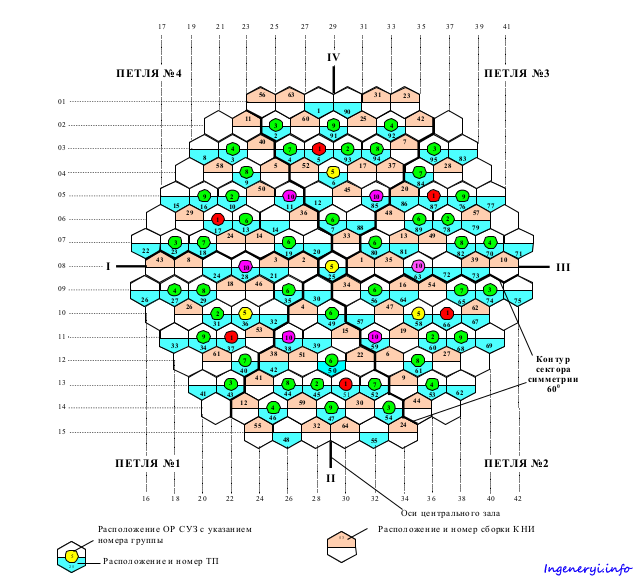
\includegraphics[width=\linewidth]{tvs}
	    \caption{Картограмма активной зоны реактора ВВЭР'1000}
	    \label{fig:my_label}
	\end{figure}
	
	\subsection{Активная зона}
	\hspace{0.4cm}
	Активная зона реактора относится к устройствам нормальной эксплуатации и к первой категории сейсмостойкости.Активная зона реактора обеспечивает выполнение следующих требований,  вытекающих  из  нормативно-технической  документации  вобласти безопасности АЭС:
	
	\begin{itemize}
	    \item 	непревышение  допустимых  пределов  повреждения  оболочек  твэлов в ТВС в пределах проектного срока службы;
	\item поддержание  требуемой  геометрии  положения  твэлов  в  ТВС  иТВС в реакторе;
	\itemвозможность осевого и радиального расширения твэлов и ТВС притемпературных и радиационных воздействиях, разности давлений,взаимодействия топливных таблеток с оболочкой;
	\item прочность  при  воздействии  механических  нагрузок  в  проектныхрежимах;
	\item выбростойкость  при  воздействии  потока  теплоносителя,  с  учетомперепада и пульсации давления, нестабильности потока, вибрации;
	\item стойкость материалов против коррозионных, электрохимических,тепловых, механических и радиационных воздействий;
	\item непревышение  проектных  значений  температуры  топлива  и  оболочки;
	\item отсутствие кризиса теплообмена в постулированных проектом режимах;
	\item стойкость СУЗ в пределах проектного ресурса от воздействия нейтронного  потока,  температуры,  перепада  и  изменения  давления,износа и ударов, связанных с перемещениями;
	\item возможность размещения внутри ТВС контролирующих датчиков;
	\item взаимозаменяемость свежих, частично и выгоревших до необходимой глубины ТВС и ПС СУЗ благодаря унификации установочныхразмеров;
	\item выполнение  критериев  аварийного  охлаждения  активной  зоны  всоответствии с действующей нормативно – технической документацией в проектных режимах;
	\item предотвращение расплавления топлива;
	\item сведения к минимуму реакции между металлом и водой;
	\item перевод  активной  зоны  в  подкритическое  состояние,  его  поддержание в пределах определенных проектом;
	\item возможность послеаварийного расхолаживания активной зоны.
	\end{itemize}
	
	Для  режимов  нормальных  условий  эксплуатации  установлен  эксплуатационный предел повреждения твэлов – за счет образования микротрещин с дефектами типа газовой неплотности оболочки не долженпревышать 0,2 \% твэлов и 0,02 \% твэлов при прямом контакте ядерного топлива с теплоносителем.
	
	Для режимов нарушения условий нормальной эксплуатации установлен предел безопасной эксплуатации твэл.
	
	Предел  безопасной  эксплуатации  по  количеству  и  величине  дефектов твэл составляет 1 \% твэлов с дефектами типа газовой неплотности и 0,1 \% твэлов, для которых имеет место прямой контакт теплоносителя ядерного топлива.Критерием  допустимости  установленных  пределов  повреждаемости твэлов является величина активности воды первого контура.В качестве эксплуатационного предела выбрано значение суммарной удельной активности радионуклидов йода 131135 в теплоносителеI контура 3,7$\cdot$10$^{8}$Бк/кг (1,0$\cdot$10$^{–3}$Ки/кг). Пределом безопасной эксплуатации  является  максимальная  суммарная  удельная  активность  радионуклидов  йода  131135  в  теплоносителе  I  контура  1,85$\cdot$10$^{8}$Бк/кг(5$\cdot$10$^{–3}$Ки/кг).  Суммарная  удельная  активность  радионуклидов  йода131135  в  теплоносителе  I  контура  должна  определяться  в  пересчёте  кпроектному расходу на очистку 30 т/ч и коэффициенте очистки фильтров по изотопам йода не менее 10.
	
	\begin{figure}
	    \centering
	    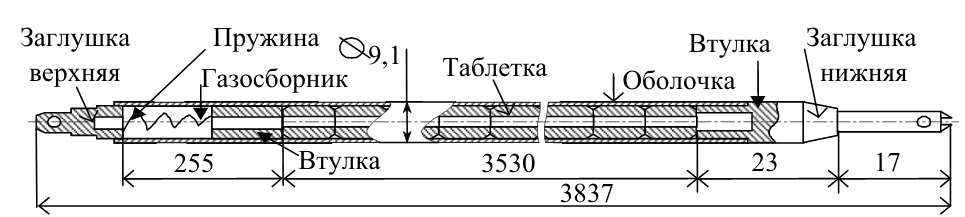
\includegraphics[width=\linewidth]{Picture1}
	    \caption{Tепловыделяющий элемент}
	    \label{fig:my_label}
	\end{figure}
	\section{Улучшение топливоиспользования в реакторах ВВЭР-1000}
	\hspace{0.4cm}
	Приоритетным  способом  улучшения  использования  топлива  на  АЭС  с  реакторами ВВЭР-1000  является  увеличение  загрузки  урана  в  ТВС и/или  повышение  обогащения топлива.  Для  ТВС  реактора  ВВЭР-1000  приняты  два  варианта  повышения  ураноемкости: увеличение  высоты  топливного  столба  при  сохранении габаритных  размеров  кассеты (тепловыделяющей сборки) и оптимизация размеров топливных таблеток и оболочек твэл. Успешная  эксплуатация ТВС-2  и  ТВСА  с  жесткими  сварными  типами  каркасов (образованными  направляющими  каналами  и  дистанционирующими  решетками  в  ТВС-2, уголками   и   дистанционирующими   решетками   в   ТВСА)   в   сочетании   с   высокой стабильностью  геометрических  характеристик  ТВС  позволила  обосновать:  возможность увеличения  загрузки  урана  в  ТВС,  безопасность  эксплуатации  ядерного  топлива  в  режиме маневрирования мощности в диапазоне 100 – 75 – 100\% Nном, работоспособность ядерного топлива  при  повышении  мощности  ВВЭР-1000  до  104\%  Nном  и  более  (до  110\% Nном). Отсутствие  ограничений  на  эксплуатационный  ресурс  с  точки  зрения  прочности  и формоизменения ТВС с жестким каркасом открыло возможности для внедрения длительных топливных  циклов,  технико-экономические  характеристики  которых  зависят  от  загрузки урана в ТВС. 
	
	
	\begin{figure}
	    \centering
	    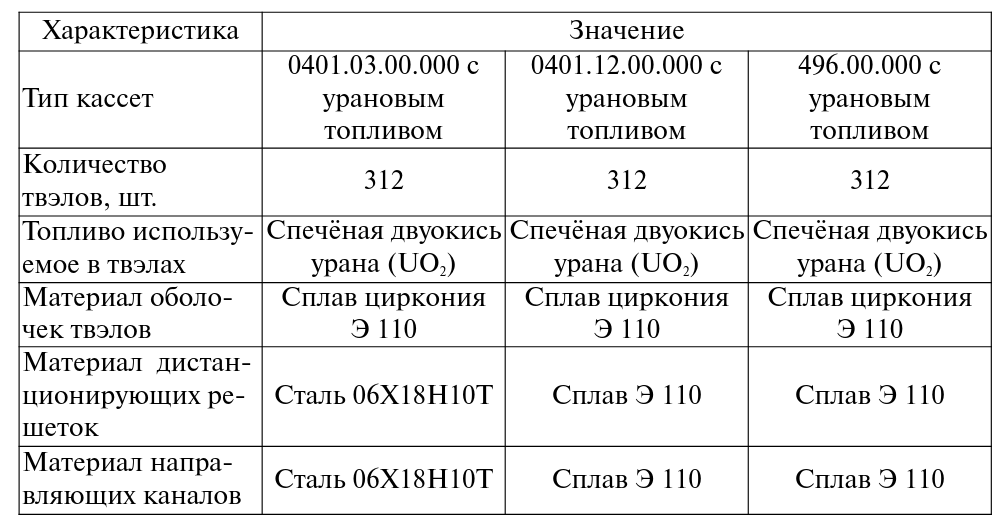
\includegraphics[width=\linewidth]{Picture2}
	    \caption{Характеристики кассет с урановым топливом}
	    \label{fig:my_label}
	\end{figure}
	
	
	\begin{figure}
	    \centering
	    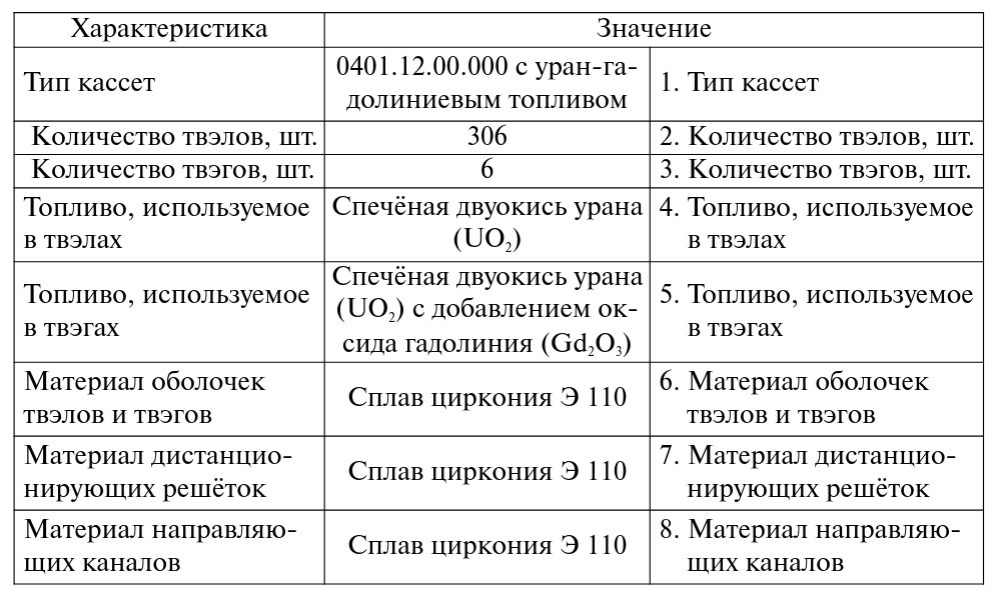
\includegraphics[width=\linewidth]{Picture3}
	    \caption{Характеристики кассет с уран-гадолиниевым топливом}
	    \label{fig:my_label}
	\end{figure}
	
	\begin{figure}
	    \centering
	    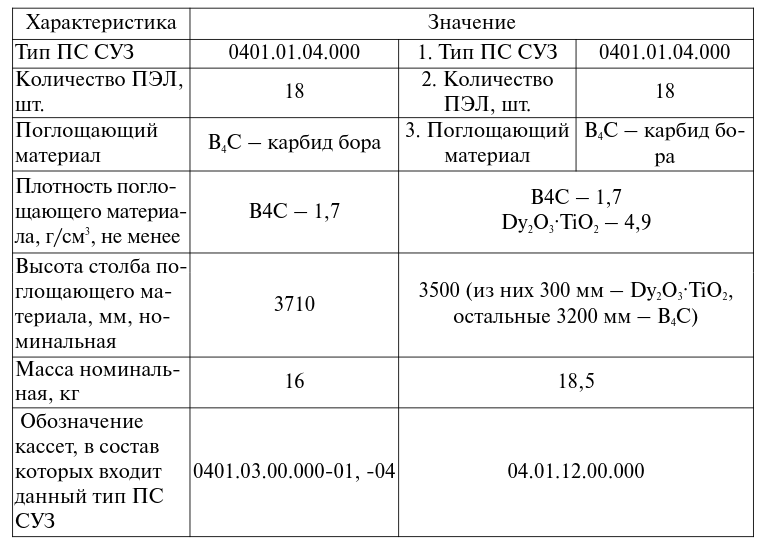
\includegraphics[width=\linewidth]{Picture4}
	    \caption{Характеристики ПС СУЗ}
	    \label{fig:my_label}
	\end{figure}
	
	\begin{figure}
	    \centering
	    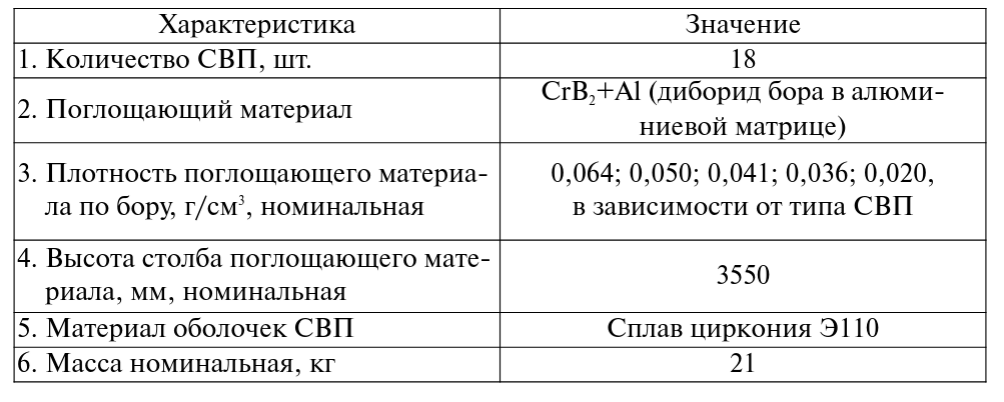
\includegraphics[width=\linewidth]{Picture5}
	    \caption{Характеристики пучков СВП}
	    \label{fig:my_label}
	\end{figure}
	
	
	Концевые  детали  ТВС  служат  для  фиксации  кассеты  в  установочных  гнездах активной  зоны.  Верхняя  концевая  деталь  (головка)  обеспечивает  взаимодействие  с внутрикорпусными устройствами реактора и поджатие ТВС от всплытия, а также разъемное соединение  с  каркасом  ТВС.  Нижняя  концевая  деталь  (хвостовик)  обеспечивает  заданное местоположение кассеты в активной зоне, а также организацию протока теплоносителя. 
	
	В настоящее время на энергоблоках Балаковской и Ростовской АЭС эксплуатируются тепловыделяющие  сборкимодификации  ТВС-2М с  увеличенным  на  150  мм  от  базового аналога топливным столбом (до 3680 мм), что позволяет обеспечить реализацию топливного цикла 3 х 18 мес. в условиях мощности АЭС, равной 104\% от номинальной. Сборки   ТВС-2   и   ТВС-2М   являются   эволюционным   развитием   конструкций предшествующих бесчехловых ТВС, по сравнению с которыми в них не добавлено ни одного нового   элемента.   Все   новые   качества   получены   путем применения   положительно зарекомендовавших  себя  в  эксплуатации  решений,  усовершенствования  конструкции отдельных составляющих элементов. На  энергоблоках  No  2  и  3  Калининской  АЭС  с  2010  года  эксплуатируются  сборки ТВСА-PLUS,  имеющие  унифицированный  с  ТВС-2М  топливный  пучок с  увеличенным  на 150 мм топливным столбом и обеспечивающие аналогичные условия эксплуатации. Загрузка урана  в  ТВС-2М  и  ТВСА-PLUS  увеличена  примерно  на  6\%  в  сравнении  с  базовыми вариантами. С 2011 года начато внедрение ТВС-2М на энергоблоке No 1 АЭС «Тяньвань» в Китае. На энергоблоке No 1 Калининской АЭС с 2006 года в пятигодичном топливном цикле эксплуатируются  кассеты  типа ТВСА-АЛЬФА  с  увеличенной  ураноемкостью  за  счет применения   твэлов   с   топливными   таблетками   без   центрального   отверстия,   с   8 дистанционирующими  решетками.  Загрузка  урана  в  ТВСА-АЛЬФА  в  сравнении  с  ТВСА увеличена на $\approx$ 10\% и составляет $ \approx$ 546 кг. Эта сборка разрабатывалась как прототип ТВС для АЭС «Темелин». 
	
	
	
	\newpage
\begin{thebibliography}{5}
\bibitem{1}Тепловыделяющая  сборка  ТВСА  ВВЭР-1000:  направления  развития  и  результаты эксплуатации / В.Б. Кайдалов [и др.] // Атомная энергия. – 2007. Т. – 102.– С. 43 – 48.

\bibitem{2}Разработка  и  внедрение  ТВС-2М  для  перспективных топливных  циклов  /  Ю.Г. Драгунов и др. // Атомная энергия. – 2005. Т. – 99.– С. 432 – 437. 
\bibitem{3}  Y.  Kovbasenko,  V.  Khalimonchuk,  A.  Kuchin,  Y.  Bilodid,  M.  Yeremenko, O. Dudka, NUREG/CR-6736, PNNL-13694 “Validation of SCALE Sequence CSAS26 for Criticality Safety Analysis of VVER and RBMK Fuel Designs”, Washington, U.S. NRC, 2002.
\bibitem{4} Optimum Cycle Length and Discharge Burnup for Nuclear Fuel: Phase II: Results Achievable with Enrichments Greater than 5.0 w/o, EPRI,  Palo  Alto,  CA  and  U.S.  Department  of Energy,  Washington,  DC: 2002. 1003217
\end{thebibliography}
	
\end{document}
